\section{Introduction}
\label{sec:introduction}

\PARstart{A}{fter} a load is restored or a line is reclosed, the machines
continue moving. A second intervention may begin before that response has
decayed. With only eight PMUs in a 39-bus network, a change in a measured
signal may therefore indicate a new source, recovery from an earlier source,
or an imperfect physical prediction. The task is to distinguish these
explanations using only the reports available at the decision time.\AIDraftingCredit{}

\begin{figure*}[t]\centering
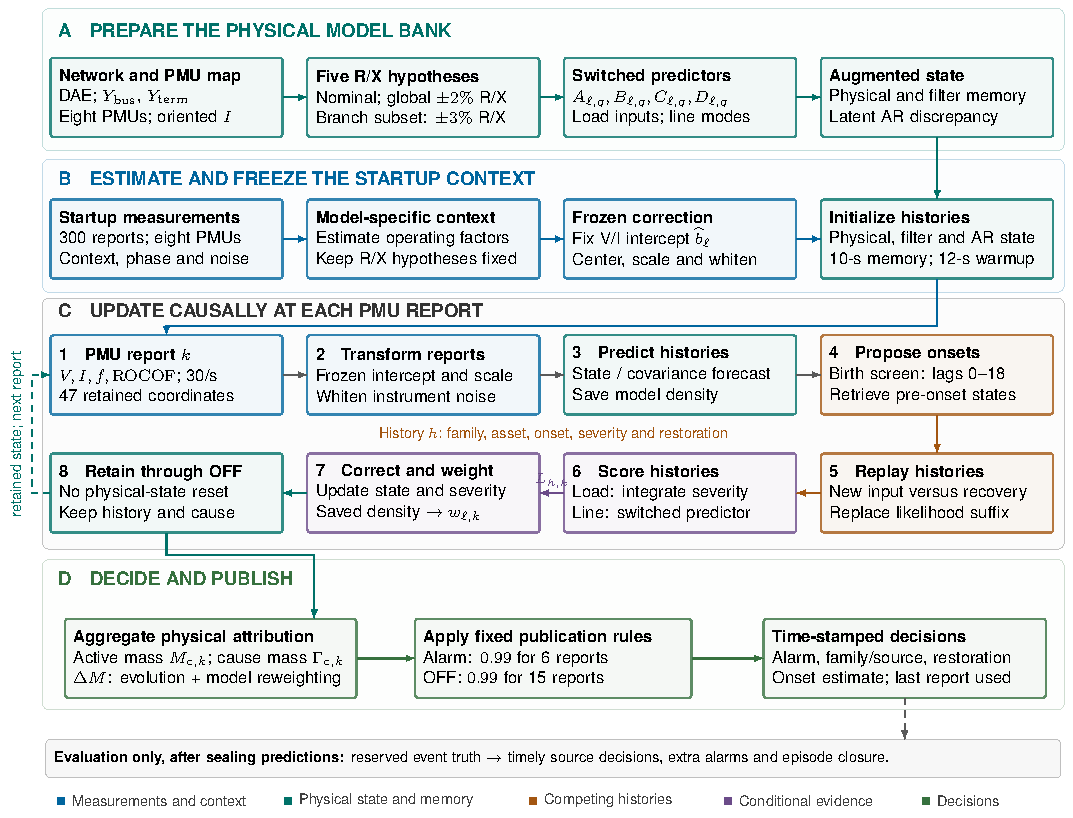
\includegraphics[width=\textwidth]{figures/generated/narrative_architecture.pdf}
\caption{Implemented physical-history attribution with its original publication policy, organized into model preparation (A), startup context (B), per-report inference (C), and publication (D). The bank predicts before state correction and saves model evidence before proposal selection. Candidate replay replaces a likelihood suffix, so each report contributes once. The feedback loop retains physical and instrumental memory through restoration. Reserved event truth is used only after predictions are sealed. The common-clock controls replace block D as specified in Section~\ref{sec:submission-checks}.}
\label{fig:joint-architecture}\end{figure*}

Physical restoration is not electrical recovery. A detector that returns
immediately to a flat reference can issue another alarm for the remaining
oscillation. Suppressing alarms throughout recovery can instead hide a real
intervention. The operating point adds another difficulty: correcting a
voltage or current offset need not correct how the network responds to a
later input.

Existing work provides strong foundations. DAE state estimators infer
unmeasured electrical states \cite{katanic2024recursive}; physical outage
detectors compare network hypotheses sequentially
\cite{chen2016quickest,rovatsos2017outage}; and simulated fault trajectories
support diagnosis from sparse PMUs \cite{warner2023highfidelity}.
Physical models, transient histories and unknown-onset searches are thus
established ingredients. A small state-reconstruction error, however, does
not by itself identify the intervention that produced the observations.

We compare physical histories rather than isolated signal features. A
history specifies an intervention, source, onset, severity and restoration.
DAE-derived predictors start from estimated past states and preserve the
state left by previous interventions. Conditional evidence integrates load
severity, accounts for instrumental memory, and updates fixed network-model
hypotheses. Separate active and cause masses keep a restored intervention
available as an explanation of the continuing response.

The paper makes three contributions within this restricted problem:
\begin{enumerate}
\item An executable attribution mechanism that makes new load/line
interventions compete with retained recovery histories. We specify its
physical predictors, evidence updates and decision rules.
\item A comparison that separates detection, correct source attribution
before restoration, extra alarms and episode closure. Nominal and uncertain
network models are evaluated alongside two fixed ExtraTrees adapters;
Chen's published detector is compared on eligible persistent line openings.
\item Adversarial tests of scope: a state-retaining physical competitor,
a classifier fitted under a grouped SIM split, and a retrospective
integrity/source replay. These tests retain failures and distinguish
simulation utility from transfer to the reference record.
\end{enumerate}

A further physical control asks whether recovery increases source separation.
It distinguishes retaining a consistent prediction from obtaining additional
information about the source; it is not a comparison of causal detectors.

On the common development cohort and publication clock, the five-model bank
obtains \SSMixTimely{}/\SSMixTotal{} timely family/source decisions with
\SSMixExtras{} extras, versus \SSSimpleTimely{}/\SSSimpleTotal{} and
\SSSimpleExtras{} for the simpler physical control. This compares complete
procedures; it does not isolate a causal effect of history retention.
\IfFileExists{generated/c01_macros.tex}{The separate
confirmatory comparison is reported below.}{The prespecified confirmatory
comparison is still running without method changes.} The claim is scoped
to the declared load/line catalog. These simulations do not establish an
all-family hackathon score, calibrated event probabilities or real-time deployment.
